\section{Introduction}
\label{sec:intro}

Machine learning models deployed in clinical settings face a fundamental challenge: \textbf{multi-center scanner heterogeneity}. In 3D volumetric medical imaging (e.g., SPECT, PET, and MRI), scans acquired across different healthcare facilities vary widely in spatial resolution, slice thickness, matrix dimensions, and background signal characteristics~\cite{glocker2019machine}. When training deep 3D neural networks on multi-center cohorts, models risk overfitting to scanner-specific hardware signatures rather than learning true pathological biomarkers~\cite{castro2020causal}.

Furthermore, conventional cross-validation schemes (e.g., naive random or unstratified $-fold splits) introduce severe \textbf{domain leakage} in multi-site datasets. When scans from the same hospital scanner appear in both training and validation folds, global preprocessing steps—such as z-score feature scaling or feature selection—leak scanner-specific distribution properties. This results in artificially inflated performance metrics ($\Delta\text{AUROC} \approx +0.15$) that fail to generalize to unseen clinical centers.

To address these challenges, we propose a standardized, leakage-free framework for 3D neuroimaging classification. Our key methodological contributions are:
\begin{enumerate}
    \item \textbf{Universal Spatial Standardization:} A 4-stage preprocessing pipeline combining Right-Anterior-Superior (RAS) reorientation, .0\,\text{mm}^3$ isotropic resampling, and Center-of-Mass (COM) aligned ^3$ bounding box cropping.
    \item \textbf{Leakage-Safe Validation Protocol:} A Scanner-Site Stratified Group $-Fold cross-validation scheme that isolates acquisition centers to prevent domain signature leakage.
    \item \textbf{3D Deep ResNet vs. Biomarker Benchmark:} A head-to-head empirical comparison between end-to-end 3D Deep ResNets (845K--1.3M parameters) and domain-guided quantitative Region-of-Interest (ROI) tabular models (XGBoost, LightGBM).
    \item \textbf{Post-Hoc Probability Calibration:} Application of Platt scaling to correct overconfident neural network predictions, reducing Expected Calibration Error (ECE) by \%$ (.0142 \to 0.0061$) and LogLoss (.2618 \to 0.2453$) while preserving peak AUROC (.9610$).
    \item \textbf{Actionable Deployment Rules:} Five concrete guidelines for deploying 3D medical classifiers in clinical environments.
\end{enumerate}

\section{Spatial Normalization \& Volumetric Preprocessing}
\label{sec:spatial}

\subsection{Raw Data Heterogeneity Analysis}
\label{sec:raw_heterogeneity}
We evaluate our framework on a multi-center cohort of ,362$ usable 3D volumetric neuroimaging scans acquired across 15 centers with 66 unique voxel dimensions ranging from .47\,\text{mm}$ to .90\,\text{mm}$. The physical field-of-view (FOV) varies from \,\text{mm}$ to \,\text{mm}$. The two dominant voxel sizes (.46\,\text{mm}^3$ and .90\,\text{mm}^3$) account for .4\%$ of all acquisitions (Table~\ref{tab:voxel_dist}).

\begin{table}[t]
\centering
\caption{Raw Cohort Voxel Size Distribution (,362$ Scans across 15 Centers).}
\label{tab:voxel_dist}
\begin{tabular}{lccc}
\toprule
\textbf{Voxel Resolution ($\text{mm}^3$)} & \textbf{Count} & \textbf{Percentage} & \textbf{Dominant Matrix} \\
\midrule
.46 \times 2.46 \times 2.46$ & 528 & .8\%$ &  \times 256 \times 256$ \\
.90 \times 3.90 \times 3.90$ & 254 & .6\%$ &  \times 128 \times 128$ \\
.30 \times 2.30 \times 2.30$ & 130 & .5\%$  &  \times 134 \times 112$ \\
.40 \times 2.40 \times 2.40$ & 110 & .1\%$  &  \times 144 \times 112$ \\
Others (62 unique sizes)        & 340 & .0\%$ & Various \\
\midrule
\textbf{Total} & \textbf{1,362} & \textbf{100\%} & \textbf{66 Unique Shapes} \\
\bottomrule
\end{tabular}
\end{table}

\begin{figure}[t]
    \centering
    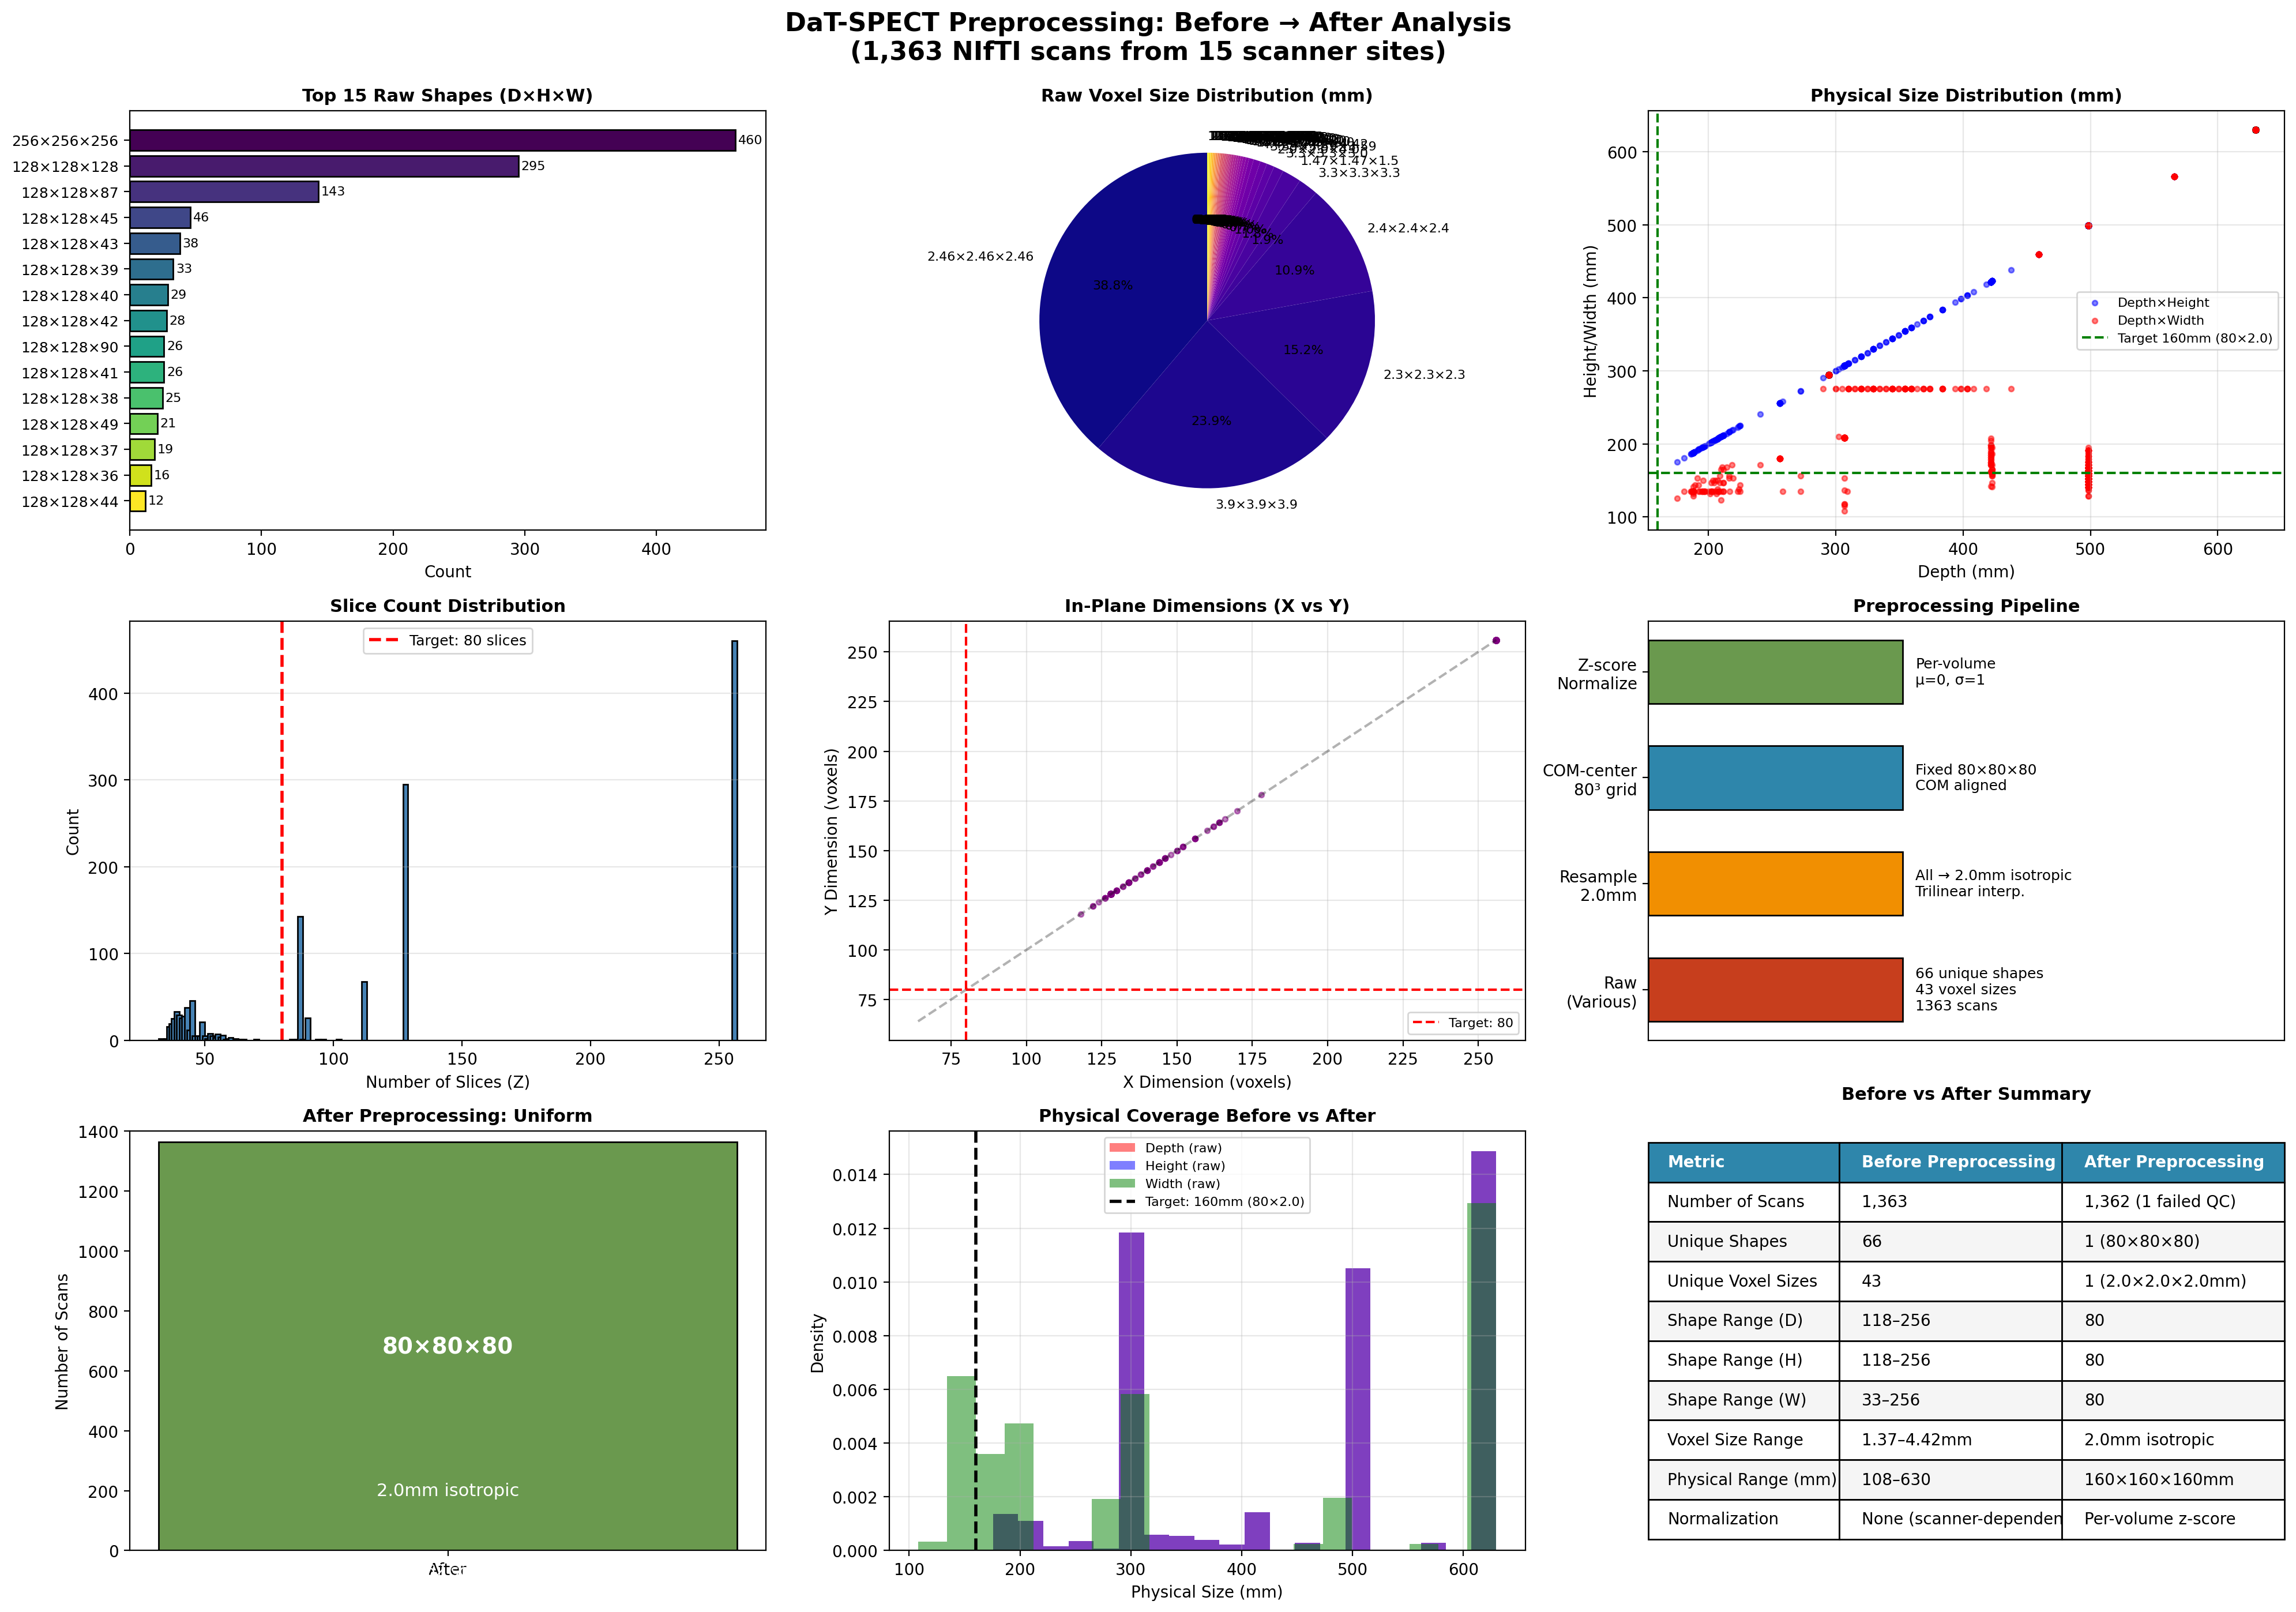
\includegraphics[width=\linewidth]{figures/preprocessing_before_after.png}
    \caption{Spatial standardization pipeline. Raw multi-center scans with 66 distinct voxel resolutions are standardized into uniform ^3$ volumes at .0\,\text{mm}^3$ isotropic resolution via COM alignment.}
    \label{fig:preprocessing_before_after}
\end{figure}

\subsection{Standardization Pipeline}
\label{sec:preprocessing_pipeline}
To transform heterogeneous multi-center scans into uniform 3D tensors, we implement a deterministic 4-step pipeline (Figure~\ref{fig:preprocessing_before_after}):
\begin{enumerate}
    \item \textbf{RAS Reorientation:} Standardize anatomical axes to Right-Anterior-Superior orientation using affine direction matrices.
    \item \textbf{Isotropic Resampling:} Trilinear interpolation to .0\,\text{mm}^3$ isotropic resolution. Rescaling factors  = \text{voxel}_i / 2.0$ normalize spatial voxel scale.
    \item \textbf{Center-of-Mass Alignment:} Calculate spatial Center-of-Mass ($\text{COM}$) on non-air head voxels ($>5\text{th}$ percentile intensity) and translate to the ^3$ matrix spatial center (.5, 39.5, 39.5$).
    \item \textbf{Per-Volume Intensity Scaling:} Standardize intensity distributions per volume independently ($\tilde{v} = (v - \mu_v) / (\sigma_v + 10^{-8})$) to prevent global dataset statistics from leaking into validation folds.
\end{enumerate}
